\documentclass[conference]{IEEEtran}
\usepackage[utf8]{inputenc}
\usepackage[brazil]{babel}
\usepackage{cite}
\usepackage{amsmath,amssymb,amsfonts}
\usepackage{algorithmic}
\usepackage{graphicx}
\usepackage{textcomp}
\usepackage{xcolor}
\usepackage{booktabs}
\usepackage{url}
\usepackage{tikz}
\usetikzlibrary{shapes.geometric, arrows, positioning}

\begin{document}

\title{Simulador de Arquitetura Multicore com Gerenciamento de Memória Paginada e Escalonamento Dinâmico de Tarefas}

\author{
    \IEEEauthorblockN{Pedro Henrique Galvão}
    \IEEEauthorblockA{\textit{DECOM-DV / CEFET-MG} \\
    devpedrohg@gmail.com}
    \and
    \IEEEauthorblockN{João Paulo}
    \IEEEauthorblockA{\textit{DECOM-DV / CEFET-MG} \\
    Divinópolis, Brasil}
    \and
    \IEEEauthorblockN{Igor Peixoto}
    \IEEEauthorblockA{\textit{DECOM-DV / CEFET-MG} \\
    Divinópolis, Brasil}
    \and
    \IEEEauthorblockN{Otávio Hiratsuka}
    \IEEEauthorblockA{\textit{DECOM-DV / CEFET-MG} \\
    Divinópolis, Brasil}
}

\maketitle

\begin{abstract}
[A SER ESCRITO PELA PESSOA 4] Lorem ipsum dolor sit amet, consectetur adipiscing elit. Sed do eiusmod tempor incididunt ut labore et dolore magna aliqua. Ut enim ad minim veniam, quis nostrud exercitation ullamco laboris nisi ut aliquip ex ea commodo consequat. Duis aute irure dolor in reprehenderit in voluptate velit esse cillum dolore eu fugiat nulla pariatur. Repositório: \url{https://github.com/PeedroHG/multicore-os-simulator}.
\end{abstract}

\begin{IEEEkeywords}
Sistemas Operacionais, Multicore, Troca de Contexto, PCB, Lockstep, Amdahl.
\end{IEEEkeywords}

\section{Introdução}
% [Seção sob responsabilidade de Otávio Hiratsuka]
Lorem ipsum dolor sit amet, consectetur adipiscing elit, sed do eiusmod tempor incididunt ut labore et dolore magna aliqua. Ut enim ad minim veniam, quis nostrud exercitation ullamco laboris nisi ut aliquip ex ea commodo consequat. Duis aute irure dolor in reprehenderit in voluptate velit esse cillum dolore eu fugiat nulla pariatur.

Excepteur sint occaecat cupidatat non proident, sunt in culpa qui officia deserunt mollit anim id est laborum. Sed ut perspiciatis unde omnis iste natus error sit voluptatem accusantium doloremque laudantium, totam rem aperiam.

\subsection{Repositório e Instruções de Compilação}
O código-fonte completo e modular do projeto está hospedado publicamente no repositório GitHub:\\
\centerline{\url{https://github.com/PeedroHG/multicore-os-simulator}}

Para a compilação e execução do simulador em ambiente GNU/Linux, utiliza-se a ferramenta Make sobre o padrão C++17:
\begin{verbatim}
# 1. Compilação do executável principal
make

# 2. Execução parametrizada do simulador
./simulador --cores 4 --politica rr --modo p

# 3. Execução da suíte completa de testes
make test

# 4. Execução da bateria de benchmarks
make benchmark
\end{verbatim}

\section{Arquitetura Multicore e Modelo de Execução}
% [Seção sob responsabilidade de Pedro Henrique Galvão]
O sistema foi estruturado com um Kernel centralizado, responsável pelo despacho e controle de tempo de $n$ núcleos de processamento idênticos ($\text{CPU}_0, \text{CPU}_1, \dots, \text{CPU}_{n-1}$). Todos os núcleos compartilham a mesma memória principal, cujo espaço físico é dividido entre a área reservada do sistema operacional (endereços $0\text{x}0000$ a $0\text{x}01\text{FF}$) e a área dos programas de usuário.

\subsection{Modelo de Execução Temporal em Lockstep}
Para afastar condições de corrida não-determinísticas inerentes à manipulação de threads assíncronas do sistema hospedeiro e assegurar reprodutibilidade experimental exata, a simulação adota o modelo de \textit{passo sincronizado} (\textit{lockstep}). 

O Kernel gerencia o relógio central do sistema através do contador \texttt{tickGlobal}. Em cada pulso de clock ($t \to t + 1$), o Kernel percorre os núcleos de $0$ a $n-1$:
\begin{enumerate}
    \item Incrementa o tempo de espera ($\text{ciclosEspera}$) de todos os processos que permanecem na fila de aptos (\texttt{PRONTO});
    \item Para núcleos em estolagem de memória, consome 1 ciclo de latência de E/S sem despachar instrução;
    \item Para núcleos desocupados, aciona o despachante para alocar o próximo processo da fila;
    \item Para núcleos com processo ativo, dispara o ciclo elementar de instrução ($\text{CPU::step()}$), atualizando registradores e o contador de quantum.
\end{enumerate}

\subsection{Bloco de Controle de Processo (PCB)}
A abstração de processo é consolidada na estrutura \texttt{PCB} (\textit{Process Control Block}), que atua como o repositório de persistência do estado lógico e arquitetural de cada tarefa admitida no lote inicial (em $t = 0$). O PCB encapsula:
\begin{itemize}
    \item \textbf{Identificação e Ciclo de Vida:} Identificador numérico exclusivo (\texttt{PID}), nome do arquivo fonte e estado formal (\texttt{NOVO}, \texttt{PRONTO}, \texttt{EXECUTANDO}, \texttt{FINALIZADO} ou \texttt{ABORTADO});
    \item \textbf{Contexto de Hardware:} Snapshot estruturado (\texttt{CPUContext}) composto pelos registradores de uso geral $R_0$ a $R_7$, Program Counter ($PC$) lógico, Instruction Register ($IR$) e sinalizadores de término da Unidade de Controle (\texttt{halted});
    \item \textbf{Descritores de Escalonamento:} Prioridade estática base, prioridade dinâmica efetiva (para mecanismos de \textit{aging}), estimativa estática de rajada e quantum consumido;
    \item \textbf{Telemetria e Métricas:} \textit{Timestamps} dos ciclos de admissão, início e encerramento, além de contadores para tempo de espera na fila, tempo de execução na CPU, tempo parado em stall e quantidade de trocas de contexto.
\end{itemize}

\subsection{Mecanismo e Penalidade de Troca de Contexto}
A troca de contexto é implementada desacopladamente na classe \texttt{CPU} através dos métodos primitivos \texttt{salvarContexto(PCB\&)} e \texttt{restaurarContexto(PCB\&)}. 

Quando um processo esgota sua fatia temporal (quantum) ou sofre preempção por prioridade, o núcleo extrai os valores dos registradores físicos e os salva no PCB. Em seguida, a CPU carrega os registradores do novo processo que vai assumir o núcleo.

Para refletir o custo operacional real de salvamento de registradores e sobrecarga do despachante~\cite{silberschatz2018}, o simulador aplica uma penalidade de tempo configurável:
\begin{equation}
C_{\text{troca}} = 5 \text{ ciclos de clock}
\end{equation}
Essa penalidade é estritamente contabilizada apenas quando há alternância efetiva de processos ($\text{PID}_{\text{anterior}} \neq \text{PID}_{\text{novo}}$) no mesmo núcleo.

\subsection{Tratamento de Faltas de Página via Estolagem (Stall)}
Em conformidade com a especificação formal do trabalho que proíbe o chaveamento de tarefas no cenário não-preemptivo, as faltas de bloco/página (\textit{page faults}) geradas pelo subsistema de memória virtual não transitam o processo para um estado tradicional \texttt{BLOQUEADO}. Em substituição, a CPU ativa um mecanismo de estolagem do núcleo (\textit{pipeline stall}) por:
\begin{equation}
C_{\text{falta}} = 50 \text{ ciclos de clock}
\end{equation}
somados a 50 ciclos adicionais caso a moldura vítima substituída exija escrita retroativa (\textit{write-back}) de dados alterados para o disco virtual. Durante os ciclos de estolagem, o núcleo permanece paralisado simulando o barramento de transferência de memória secundária, garantindo fidelidade temporal ao cenário não-preemptivo.

\subsection{Fluxograma Geral da Arquitetura}
O fluxo operacional do Kernel e a interação síncrona entre núcleos, despachante e memória estão esquematizados na Figura~\ref{fig:fluxograma_sistema}.

\begin{figure}[htbp]
\centering
\begin{tikzpicture}[node distance=1.3cm, auto,
    block/.style={rectangle, draw, fill=blue!10, text width=6.5cm, text centered, rounded corners, minimum height=0.8cm, font=\small},
    decision/.style={diamond, draw, fill=orange!10, text width=4.0cm, text centered, font=\footnotesize, inner sep=0pt},
    line/.style={draw, -latex', thick}]
    
    \node [block] (init) {Admissão do Lote Fechado ($t = 0$) $\to$ Criação dos PCBs};
    \node [block, below of=init] (tick) {Avanço do Relógio Central: $\text{tickGlobal} \to \text{tickGlobal} + 1$};
    \node [block, below of=tick] (loop) {Kernel itera sobre núcleos $k = 0 \dots n-1$};
    \node [decision, below of=loop, node distance=1.7cm] (stall) {Núcleo $k$ em Stall (Page Fault)?};
    \node [block, right of=stall, node distance=3.2cm, fill=red!10, text width=2.2cm] (decstall) {Decrementa stall; stall++};
    \node [decision, below of=stall, node distance=1.8cm] (idle) {Núcleo $k$ Livre?};
    \node [block, right of=idle, node distance=3.2cm, fill=green!10, text width=2.2cm] (alloc) {Despachante: restaura PCB};
    \node [block, below of=idle, node distance=1.6cm] (step) {Executa Instrução: $\text{CPU}_k\text{::step()}$};
    \node [decision, below of=step, node distance=1.7cm] (halt) {Instrução HALT encontrada?};
    \node [block, right of=halt, node distance=3.2cm, fill=gray!20, text width=2.2cm] (finish) {PCB FINALIZADO; Libera núcleo};
    \node [decision, below of=halt, node distance=1.8cm] (preempt) {Quantum esgotado (Modo P)?};
    \node [block, right of=preempt, node distance=3.2cm, fill=yellow!20, text width=2.2cm] (save) {Salva PCB; Devolve à fila};
    \node [decision, below of=preempt, node distance=1.8cm] (active) {Existem tarefas pendentes?};
    \node [block, below of=active, node distance=1.6cm, fill=green!20] (end) {Término da Simulação (Makespan final)};

    \path [line] (init) -- (tick);
    \path [line] (tick) -- (loop);
    \path [line] (loop) -- (stall);
    \path [line] (stall) -- node [above] {Sim} (decstall);
    \path [line] (stall) -- node [right] {Não} (idle);
    \path [line] (idle) -- node [above] {Sim} (alloc);
    \path [line] (idle) -- node [right] {Não} (step);
    \path [line] (alloc) |- (step);
    \path [line] (step) -- (halt);
    \path [line] (halt) -- node [above] {Sim} (finish);
    \path [line] (halt) -- node [right] {Não} (preempt);
    \path [line] (preempt) -- node [above] {Sim} (save);
    \path [line] (preempt) -- node [right] {Não} (active);
    \path [line] (decstall) |- (active);
    \path [line] (finish) |- (active);
    \path [line] (save) |- (active);
    \path [line] (active) -- node [right] {Não} (end);
    \path [line] (active.west) -- ++(-1.0,0) |- node [near start, above] {Sim} (tick.west);
\end{tikzpicture}
\caption{Fluxograma do ciclo de execução multicore em passo sincronizado (Lockstep) gerenciado pelo Kernel.}
\label{fig:fluxograma_sistema}
\end{figure}

\section{Gerenciamento de Memória Virtual}
% [Seção sob responsabilidade de João Paulo: Fatiamento em 16 palavras, MMU, Tabela de Molduras, FIFO e LRU]

Embora o enunciado empregue a expressão ``memória segmentada'', os mecanismos prescritos --- divisão do espaço em blocos de tamanho fixo combinados a deslocamento (\textit{offset}) e substituição por FIFO ou LRU --- caracterizam formalmente a \textbf{paginação sob demanda} no modelo clássico de Tanenbaum~\cite{tanenbaum2015}. Para viabilizar a multiprogramação sem colisão de endereços entre núcleos, a Unidade de Controle (UC) foi desacoplada da memória física: o Contador de Programa ($PC$) de todo processo inicia em $0\text{x}000$, a soma estática de \texttt{OS\_RESERVED\_MEM} ($512$) foi eliminada das instruções \texttt{LOAD}, \texttt{STORE}, \texttt{BEQ} e \texttt{JUMP}, e todos os acessos --- inclusive a busca de instruções (\textit{fetch}) --- são interceptados pela Unidade de Gerenciamento de Memória (MMU).

\subsection{Fatiamento de Bits e Espaço de Endereçamento}
Na arquitetura RISC de 16 bits adotada, as instruções do tipo I (\texttt{LOAD}, \texttt{STORE} e \texttt{BEQ}) dispõem de 8 bits de endereço imediato ($0\text{x}00$--$0\text{xFF}$), ao passo que desvios incondicionais (\texttt{JUMP}) alcançam 12 bits ($0\text{x}000$--$0\text{xFFF}$). Caso fossem empregadas páginas grandes (e.g., 64 ou 256 palavras), programas inteiros caberiam em uma única página, tornando indistinguíveis as políticas de substituição. Adotou-se, portanto, o tamanho de página $P = 2^4 = 16$ palavras, estabelecendo o fatiamento exibido na Tabela~\ref{tab:fatiamento_mmu}:

\begin{table}[htbp]
\caption{Fatiamento de Endereços Lógicos e Físicos na MMU}
\label{tab:fatiamento_mmu}
\centering
\footnotesize
\begin{tabular}{@{}llll@{}}
\toprule
\textbf{Endereço} & \textbf{Largura} & \textbf{Fatiamento de Bits} & \textbf{Capacidade} \\
\midrule
Lógico  & 12 bits & $[11:4]$ página (8b) $\mid$ $[3:0]$ offset (4b) & 256 págs. $\times$ 16 pal. \\
Físico  & 16 bits & $[15:4]$ moldura (12b) $\mid$ $[3:0]$ offset (4b) & 4096 molduras (64K) \\
\bottomrule
\end{tabular}
\end{table}

Endereços lógicos com bits $[15:12] \neq 0$ ultrapassam o limite de 4096 palavras ($0\text{x}0\text{FFF}$) e disparam falha de segmentação (\texttt{SEGFAULT}), abortando o processo infrator sem interromper o lote. Dado um endereço lógico $e$, a página $p$, o deslocamento $d$ e o endereço físico $e_f$ associado à moldura física $m$ são obtidos em tempo constante por operações bit a bit:
\begin{equation}
p = e \gg 4, \quad d = e \mathbin{\&} \text{0x000F}, \quad e_f = (m \ll 4) \mathbin{|} d
\end{equation}

As primeiras $\text{MOLDURAS\_SO} = 512 / 16 = 32$ molduras físicas (endereços $0\text{x}0000$ a $0\text{x}01\text{FF}$) permanecem estritamente reservadas ao núcleo do Sistema Operacional. Os processos de usuário compartilham um conjunto configurável de $M \in [4, 32]$ molduras físicas ($m = 32 + i$, com $0 \le i < M$), impondo escassez controlada de RAM para exercitar a paginação.

\subsection{Tabela de Páginas, Core Map e Paginação sob Demanda}
O isolamento entre espaços virtuais é assegurado por três estruturas complementares:
\begin{enumerate}
    \item \textbf{Tabela de Páginas por Processo (\texttt{PCB::tabelaPaginas}):} Vetor de 256 descritores \texttt{EntradaPagina} embutido no próprio PCB (atuando de forma análoga ao registrador base \textit{PTBR}). Cada entrada mantém os bits de presença (\texttt{valida}), modificação (\texttt{suja} / \textit{dirty bit}), referência (\texttt{referenciada}) e o índice da \texttt{moldura} física correspondente;
    \item \textbf{Tabela de Molduras Global (\textit{Core Map}):} Vetor de $M$ descritores que rastreia o estado de ocupação de cada quadro de usuário (\texttt{livre}, \texttt{pid} proprietário, número da \texttt{pagina}, ordem de carga \texttt{carregadaEm} e carimbo temporal \texttt{ultimoAcesso});
    \item \textbf{Disco Virtual por Processo:} Na admissão do lote ($t = 0$), o \texttt{RAMLoader} constrói a imagem lógica de 4096 palavras de cada tarefa diretamente no disco virtual simulado, sem tocar na RAM física, e inicializa todas as 256 páginas do PCB com $\texttt{valida} = \text{falso}$.
\end{enumerate}

Quando um núcleo requisita uma palavra cuja página encontra-se inválida, ocorre uma \textbf{falta de página} (\textit{page fault}). A MMU aloca a moldura livre de menor índice ou, na ausência de quadros vagos, aciona o algoritmo de substituição global~\cite{tanenbaum2015}, podendo selecionar vítimas pertencentes a qualquer processo ativo. Se a página vítima possuir $\texttt{suja} = \text{verdadeiro}$ (modificada por instrução \texttt{STORE}), seus 16 endereços são copiados de volta para a imagem no Disco Virtual (\textit{write-back}) antes da carga da nova página. A penalidade em ciclos devolvida ao núcleo é dada por:
\begin{equation}
C_{\text{stall}} = \begin{cases}
0, & \text{se } \texttt{valida} = \text{verdadeiro (Hit)} \\
C_{\text{falta}}, & \text{se falta com moldura livre ou vítima limpa} \\
2 \cdot C_{\text{falta}}, & \text{se falta com vítima suja (\textit{write-back})}
\end{cases}
\end{equation}
onde $C_{\text{falta}} = 50$ ciclos. Ao término ou aborto de um processo, todas as suas molduras são liberadas no \textit{Core Map}.

\subsection{Políticas de Substituição Global: FIFO, LRU e OPT}
Foram implementadas duas políticas online na MMU e um oráculo offline de avaliação:
\begin{itemize}
    \item \textbf{FIFO (\textit{First-In, First-Out}):} Mantém uma fila circular de índices de molduras na ordem estrita de carregamento (\texttt{contadorCargas}). Substitui a página residente há mais tempo, independentemente de sua frequência de uso, estando sujeito à Anomalia de Belady~\cite{belady1969};
    \item \textbf{LRU Exato (\textit{Least Recently Used}):} A cada acesso (busca, leitura ou escrita), a MMU incrementa um \textbf{contador monotônico global de acessos} (\texttt{contadorAcessos}) e registra-o em \texttt{ultimoAcesso} da moldura. O uso de um contador de eventos em vez do \texttt{tickGlobal} elimina empates quando múltiplos núcleos acessam a memória no mesmo pulso de clock. Como algoritmo de pilha, o LRU satisfaz a propriedade de inclusão de Mattson et al.~\cite{mattson1970} e é imune à Anomalia de Belady;
    \item \textbf{OPT de Belady (Offline):} A MMU exporta o rastro completo de referências $(t, \text{core}, \text{PID}, p, \text{tipo})$ em CSV, processado pelo script \texttt{scripts/opt\_belady.py} para substituir a página cujo próximo uso está mais distante no futuro~\cite{belady1966}, estabelecendo o limite inferior teórico de faltas.
\end{itemize}

O fluxo completo de tradução de endereços, detecção de faltas e substituição com escrita retroativa está ilustrado na Figura~\ref{fig:fluxograma_mmu}.

\begin{figure}[htbp]
\centering
\begin{tikzpicture}[node distance=1.15cm, auto,
    block/.style={rectangle, draw, fill=blue!10, text width=5.6cm, text centered, rounded corners, minimum height=0.65cm, font=\scriptsize},
    decision/.style={diamond, draw, fill=orange!10, text width=3.2cm, text centered, font=\scriptsize, inner sep=0pt},
    line/.style={draw, -latex', thick}]

    \node [block] (req) {Requisição à MMU: $(\text{PID}, e_{\text{lógico}}, \text{R/W/X})$};
    \node [decision, below of=req, node distance=1.35cm] (seg) {$e_{\text{lógico}} > \text{0x0FFF}$?};
    \node [block, right of=seg, node distance=3.2cm, fill=red!15, text width=1.9cm] (abort) {SEGFAULT (Aborta PCB)};
    \node [block, below of=seg, node distance=1.35cm] (split) {Fatiamento: $p = e \gg 4$, $d = e \mathbin{\&} \text{0xF}$};
    \node [decision, below of=split, node distance=1.35cm] (hit) {$\text{TP}[p].\text{valida}$?};
    \node [block, right of=hit, node distance=3.2cm, fill=green!15, text width=1.9cm] (okhit) {Hit ($C_{\text{stall}}=0$)};
    \node [block, below of=hit, node distance=1.4cm, fill=yellow!15] (fault) {Page Fault: busca moldura livre ou vítima (FIFO/LRU)};
    \node [decision, below of=fault, node distance=1.45cm] (dirty) {Vítima $\text{suja}$?};
    \node [block, right of=dirty, node distance=3.2cm, fill=red!10, text width=1.9cm] (wb) {Write-back ($+50$ ciclos)};
    \node [block, below of=dirty, node distance=1.45cm] (load) {Copia página do Disco Virtual $\to$ RAM ($+50$ ciclos)};
    \node [block, below of=load, node distance=1.1cm, fill=green!20] (done) {Atualiza bits R/M e LRU; acessa $\text{RAM}[(m \ll 4)|d]$};

    \path [line] (req) -- (seg);
    \path [line] (seg) -- node [above, font=\scriptsize] {Sim} (abort);
    \path [line] (seg) -- node [right, font=\scriptsize] {Não} (split);
    \path [line] (split) -- (hit);
    \path [line] (hit) -- node [above, font=\scriptsize] {Sim} (okhit);
    \path [line] (hit) -- node [right, font=\scriptsize] {Não} (fault);
    \path [line] (fault) -- (dirty);
    \path [line] (dirty) -- node [above, font=\scriptsize] {Sim} (wb);
    \path [line] (dirty) -- node [right, font=\scriptsize] {Não} (load);
    \path [line] (wb) |- (load);
    \path [line] (load) -- (done);
    \path [line] (okhit) |- (done);
\end{tikzpicture}
\caption{Fluxograma de tradução de endereços, tratamento de falta de página e substituição na MMU.}
\label{fig:fluxograma_mmu}
\end{figure}

\section{Políticas de Escalonamento de Tarefas}
% [Seção sob responsabilidade de Igor Peixoto: FCFS, SJN, RR, Prioridade + Aging e Pseudocódigos Formais]

\section{Metodologia Experimental e Cargas de Teste}
% [Seção sob responsabilidade de Otávio Hiratsuka: Lotes CPU-bound, Memory-bound e Misto]

\section{Resultados e Discussão}

\subsection{Análise de Speedup e Escalabilidade Multicore (Experimento E1)}
A quantificação do ganho advindo da paralelização física do hardware toma como referência a formulação clássica da Lei de Amdahl~\cite{amdahl1967}. O Speedup $S(n)$ sobre $n$ núcleos de processamento é mensurado comparando o makespan (tempo total de conclusão do lote) obtido na configuração uniprocessada $T(1)$ contra a execução paralela em $n$ núcleos $T(n)$:
\begin{equation}
S(n) = \frac{T(1)}{T(n)}
\end{equation}

A eficiência paralela normalizada $E(n)$, que traduz a fração de hardware efetivamente convertida em aceleração líquida, é definida por:
\begin{equation}
E(n) = \frac{S(n)}{n} \times 100\%
\end{equation}

% [Os gráficos comparativos e a discussão aprofundada dos resultados serão inseridos após a execução completa dos benchmarks com os lotes finais de teste.]

\subsection{Desempenho da Paginação: FIFO vs. LRU vs. OPT e Anomalia de Belady (Experimento E4)}
% [Análise do Experimento E4 sob responsabilidade de João Paulo (Pessoa 2)]
Para avaliar o subsistema de memória virtual sob diferentes graus de pressão de RAM, o Experimento E4 submeteu um lote de 6 processos (totalizando $1.150$ referências à memória e conjunto de trabalho agregado de 25 páginas lógicas distintas, combinando varreduras cíclicas e laços com localidade temporal~\cite{denning1968}) à variação da quantidade de molduras de usuário $M \in \{4, 6, 8, 12, 16, 24, 32\}$, contrastando as políticas FIFO, LRU e o limite ótimo offline (OPT de Belady). A Tabela~\ref{tab:resultados_e4} sintetiza as faltas de página obtidas nos cenários uniprocessado ($n = 1$, sem entrelaçamento entre processos) e multiprocessado ($n = 4$, com competição simultânea pelas molduras globais).

\begin{table}[htbp]
\caption{Faltas de Página e Taxa de Faltas em Função do Número de Molduras ($1.150$ Referências)}
\label{tab:resultados_e4}
\centering
\footnotesize
\begin{tabular}{@{}rrrrrrr@{}}
\toprule
 & \multicolumn{3}{c}{\textbf{Single-Core ($n=1$)}} & \multicolumn{3}{c}{\textbf{Multicore ($n=4$ núcleos)}} \\
\cmidrule(lr){2-4} \cmidrule(lr){5-7}
\textbf{$M$} & \textbf{FIFO} & \textbf{LRU} & \textbf{OPT} & \textbf{FIFO} & \textbf{LRU} & \textbf{OPT} \\
\midrule
4  & 308 (26,8\%) & 303 (26,3\%) & 185 (16,1\%) & 553 (48,1\%) & 507 (44,1\%) & 357 (31,0\%) \\
6  & 308 (26,8\%) & 226 (19,7\%) &  89 (7,7\%)  & 455 (39,6\%) & 361 (31,4\%) & 258 (22,4\%) \\
8  &  25 (2,2\%)  &  25 (2,2\%)  &  25 (2,2\%)  & 364 (31,7\%) & 307 (26,7\%) & 200 (17,4\%) \\
12 &  25 (2,2\%)  &  25 (2,2\%)  &  25 (2,2\%)  & 294 (25,6\%) & 258 (22,4\%) & 128 (11,1\%) \\
16 &  25 (2,2\%)  &  25 (2,2\%)  &  25 (2,2\%)  & 157 (13,7\%) & 185 (16,1\%) &  70 (6,1\%)  \\
24 &  25 (2,2\%)  &  25 (2,2\%)  &  25 (2,2\%)  &  28 (2,4\%)  &  26 (2,3\%)  &  25 (2,2\%)  \\
32 &  25 (2,2\%)  &  25 (2,2\%)  &  25 (2,2\%)  &  25 (2,2\%)  &  25 (2,2\%)  &  25 (2,2\%)  \\
\bottomrule
\end{tabular}
\end{table}

A análise dos dados experimentais e da curva apresentada na Figura~\ref{fig:e4_faltas} evidencia quatro fenômenos centrais da teoria de memória virtual:
\begin{enumerate}
    \item \textbf{Superioridade do LRU sob Localidade Temporal:} Em $n = 1$ com $M = 6$ molduras, o FIFO permanece estagnado em $308$ faltas ($26,8\%$), pois expulsa ciclicamente a página de código do laço interno quente pelo simples fato de ela ter sido carregada no início do processo. O LRU preserva as páginas recentemente referenciadas e reduz as faltas para $226$ ($-26,6\%$). Em $n = 4$ com $M = 6$, o LRU evita $94$ faltas em relação ao FIFO ($361$ contra $455$, redução de $20,7\%$);
    \item \textbf{Pressão de Memória Multicore e \textit{Thrashing}:} Enquanto no modo sequencial ($n = 1$) $M = 8$ molduras bastam para acomodar o \textit{working set}~\cite{denning1968} individual de cada tarefa e atingir o piso de $25$ faltas compulsórias (\textit{cold-start misses}, $2,17\%$), na execução paralela em $n = 4$ núcleos quatro processos disputam simultaneamente o \textit{Core Map} global. Com $M = 4$ (apenas 1 moldura por núcleo ativo), a taxa de faltas no FIFO atinge $48,1\%$ ($553$ faltas e $82$ \textit{write-backs}), caracterizando \textit{thrashing}; o piso de faltas compulsórias só é alcançado quando $M \ge 24$ comporta a soma dos conjuntos de trabalho concorrentes;
    \item \textbf{Padrões Cíclicos e Distância para o Ótimo (OPT):} Em $n = 4$ e $M = 16$, observa-se o caso clássico descrito por Silberschatz~\cite{silberschatz2018} em que uma varredura cíclica ligeiramente maior que o número de molduras disponíveis penaliza o LRU ($185$ faltas) frente ao FIFO ($157$ faltas), ao passo que o algoritmo clarividente OPT de Belady reduz as faltas para apenas $70$ ($6,1\%$), comprovando seu papel como limite inferior inatingível por políticas puramente causais;
    \item \textbf{Verificação da Anomalia de Belady:} Submetendo a cadeia canônica de Belady et al.~\cite{belady1969} ($\langle 1,2,3,4,1,2,5,1,2,3,4,5 \rangle$) à MMU implementada e ao verificador \texttt{opt\_belady.py}, constatou-se que a ampliação de $M = 3$ para $M = 4$ molduras \textbf{eleva} as faltas do FIFO de $9$ para $10$, ao passo que no LRU as faltas caem monotonicamente de $10$ para $8$ (e no OPT de $7$ para $6$), confirmando empiricamente a propriedade de inclusão dos algoritmos de pilha~\cite{mattson1970}.
\end{enumerate}

\begin{figure}[htbp]
\centering
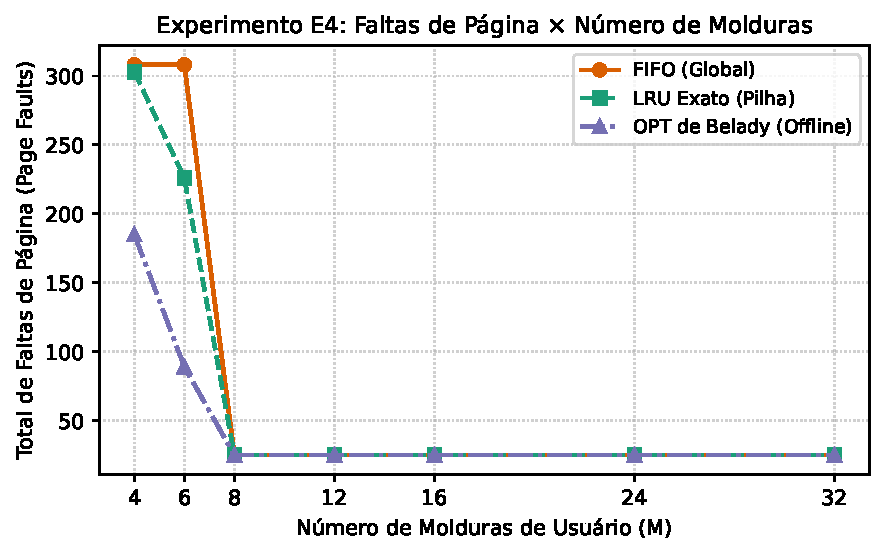
\includegraphics[width=0.98\columnwidth]{fig_e4_faltas.pdf}
\caption{Curva de faltas de página em função do número de molduras de usuário ($M$) para FIFO, LRU e OPT de Belady (Experimento E4).}
\label{fig:e4_faltas}
\end{figure}

\section{Conclusão}
% [Seção sob responsabilidade de Otávio Hiratsuka]
Lorem ipsum dolor sit amet, consectetur adipiscing elit. Sed do eiusmod tempor incididunt ut labore et dolore magna aliqua. Ut enim ad minim veniam, quis nostrud exercitation ullamco laboris nisi ut aliquip ex ea commodo consequat. Duis aute irure dolor in reprehenderit in voluptate velit esse cillum dolore eu fugiat nulla pariatur.

\bibliographystyle{IEEEtran}
\bibliography{referencias}

\end{document}
